\documentclass[]{article}
\usepackage{amsmath}
\usepackage{amssymb}
\usepackage{graphicx}
\usepackage{listings}
\usepackage{color}
\usepackage{hyperref}


% commands
\newcommand{\bra}[1]{\left\langle #1 \right|}
\newcommand{\ket}[1]{\left| #1 \right\rangle}
\newcommand{\braket}[2]{\left\langle #1 \middle| #2 \right\rangle}
\newcommand{\s}[1]{\left\{ #1 \right\}}
\newcommand{\p}[1]{\left( #1 \right)}
\newcommand{\bk}[1]{\left[ #1 \right]}
\newcommand{\w}[1]{\mathbf{#1}}
\newcommand{\parfr}[2]{\frac{\partial #1}{\partial #2}}
\newcommand{\ZZ}{\mathbb{Z}}
\newcommand{\II}{\mathbb{I}}
\newcommand{\RR}{\mathbb{R}}
\newcommand{\CC}{\mathbb{C}}
\newcommand{\Kp}{\mathcal{K}}

% math operators
\DeclareMathOperator\arctanh{arctanh}
\DeclareMathOperator\Tr{Tr}


%opening
\title{Introduction to the Koopman Operator, the VAMP Score, and VAMPNets}
\author{Phillip Bement}

\begin{document}

\maketitle

\section{The Koopman Operator}

\subsection{defining the Koopman operator}

Consider any Markov chain. Examples of Markov chains:

$\bullet$ A Markov chain with a finite number of states. The probabilities for the transitions between states are given by the stochastic transition matrix $\w{S}$.

$\bullet$ Brownian motion. Here the number of states is infinite. Time is continuous, so to get an actual Markov chain, we pick a discrete time step $\Delta t$ and only look at the particle in evenly spaced intervals of $\Delta t$ to see how it has moved.

$\bullet$ Classical dynamics on a continuous phase space. Again, we have to pick a time spacing $\Delta t$. Deterministic dynamics are a special case of stochastic dynamics.

$\bullet$ Dynamics of a polymer interacting with its environment. This is like classical dynamics, but with randomness introduced because of the interaction with the environment. Again, we still need to introduce a $\Delta t$. Often, the polymer is modelled as occupying a finite volume, often a box with cyclic boundary conditions.

From the last 3 examples, we can see that most systems we encounter in physics can be modelled as Markov chains.

If we are lucky, the dynamics of the system we are studying will be linear. This makes the system easier (or in many cases, {\em possible at all}) to solve analytically. But some systems have non-linear dynamics. The non-linear dynamics make them quite difficult to study.

The Koopman operator approach gives us a way around this issue: We can linearize the problem by considering functions on the state space rather than individual states in the state space. This trick comes with a cost. But first we should describe the trick itself.

Suppose that states of the system are denoted by points $\w{x}\in X$ where $X$ is the set of all possible system states (in classical physics, it might represent the phase space of the system). Then the Markov chain dynamics are defined by a probability (density) $p(\w{x}_{t+1}|\w{x}_{t})$. To define the Koopman operator, we should then start considering the vector space $\CC^X$, the space of functions on $X$.

\begin{figure}[h!]
	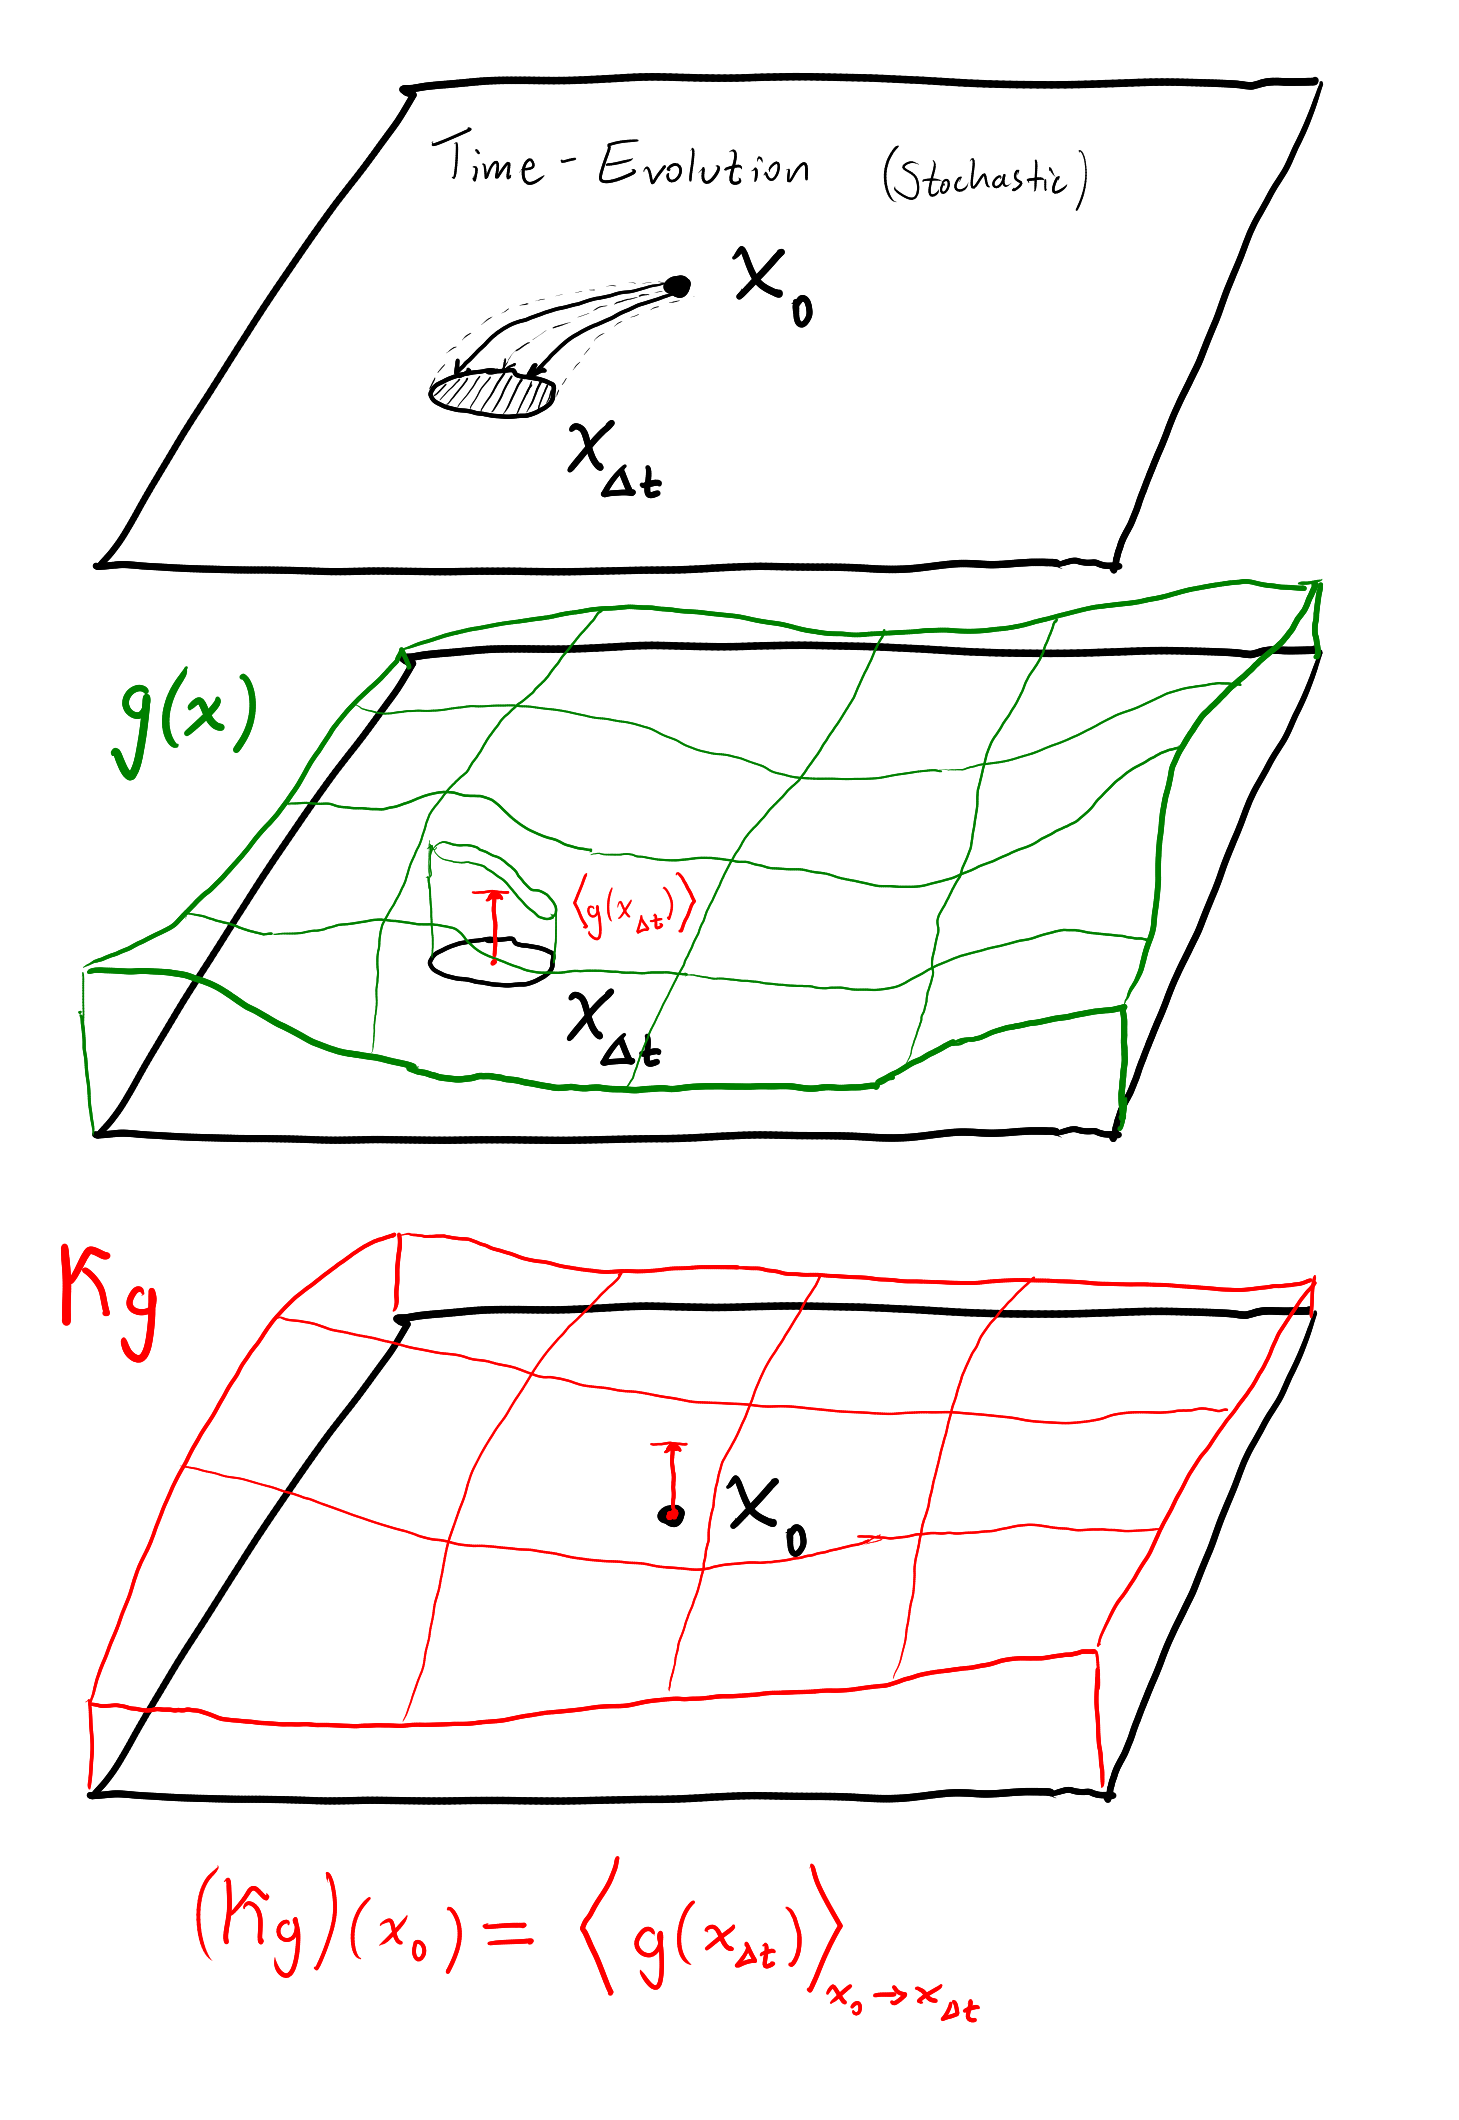
\includegraphics[width=\textwidth]{koopman_definition_diagram.png}
\end{figure}

Let $g:X\to\CC$ be any function on system states. Say that we know the system state at time $t$ is $\w{x}_t$. Then $g(\w{x}_t)$ is known. Now suppose we allow the system to evolve for time $\Delta t$ to state $\w{x}_{t+\Delta t}$. In general this evolution is stochastic. Then it turns out that we can think of $\langle g(\w{x}_{t+\Delta t})\rangle$ itself as some function of $\w{x}_t$.

Then there is some operator $\Kp$ that maps $g$ to $\langle g(\w{x}_{t+\Delta t})\rangle$. Using the transition probabilities, we can write this as follows:

$$
(\Kp g)(\w{x}) = \int_X d\w{y} p(\w{y}|\w{x}) g(\w{y})
$$

By inspecting this formula, we can see that $\Kp g$ considered as a function/vector is indeed linear in $g$.

Our first example was the Markov chain on a finite state space $X$, with a stochastic transition matrix $\w{S}$. For any given function $g:X \to \CC$, the Koopman operator acts like this:

$$
(\Kp g)(x) = \sum_{y\in X} g(y) S_{xy}
$$

We can event treat the functions as being vectors in $\CC^{|X|}$, and then writing this as a vector matrix product gives:

$$
\Kp \w{g} = \w{S}\w{g}
$$


\subsection{the cost of using Koopman theory}

In general Koopman theory is useful because it turns even a system with chaotic or non-linear dynamics into a linear operator. We can then diagonalize the operator, or take the singular value decomposition to get insight into the system.

As for the drawbacks, consider Brownian motion, our second example of a Markov chain above. It takes 3 real numbers to describe the current state of the system: We just need to write down the position of the particle. But the Koopman operator does not operate on positions, but on functions on the space. It takes infinitely many real numbers to describe such a function (for example, by telling you what its Fourier coefficients are).

Similarly, in a finite state space context, functions are vectors. And if it takes $n$ bits of information to describe which state the system is in, the vectors live in a $2^n$ dimensional space. So using Koopman theory comes with an exponential cost. (This is akin to the situation in statistics/quantum mechanics where the probability distribution/wavefunction takes an exponential amount of data to describe. To carry the analogy with quantum mechanics further, the Koopman operator itself would be the classical analogue of the unitary time-evolution operator.)


\subsection{equilibrium and inner products}

Some Markov chains approach an equilibrium if you let them evolve for long enough. Some do not. For example, in classical mechanics, the dynamics are reversible, so that even after a large amount of time, the starting conditions can still be deduced by just looking at the current state of the system. So classical physics is not a case where equilibrium is approached. The fact that the dynamics is deterministic and reversible prevents it. Brownian motion is not deterministic, but it also does not have an equilibrium distribution. The variance of the particle position increases without bound.

A polymer interacting with its environment (our 4th example above) will approach an equilibrium distribution, $q$.

In general, an equilibrium distribution $q$ must satisfy the following fixed point equation:

$$
q(\w{x}) = \int_X d\w{y} q(\w{y}) p(\w{x}|\w{y})
$$

\iffalse

$$
\int_X d\w{z}
\delta(\w{x}-\w{z})
q(\w{x})
= \int_X d\w{z}
\delta(\w{x}-\w{z})
\int_X d\w{y} q(\w{y}) p(\w{x}|\w{y})
$$

$$
q(\w{x})
=
\int_X d\w{y} q(\w{y})
\int_X d\w{z} \delta(\w{x}-\w{z})
p(\w{z}|\w{y})
$$

$$
q(\w{x})
=
\int_X d\w{y} q(\w{y})
\p{\Kp\hspace{0.2cm} \lambda\w{z}.\delta(\w{x}-\w{z})}(\w{y})
$$

\fi

For systems that do indeed approach equilibrium, this should uniquely define $q$ once we impose positivity and normalization. (In the case of classical physics, there are multiple solutions $q$ of the fixed point equation, so there is no unique equilibrium distribution. In the case of Brownian motion, there is a unique solution, $q(\w{x}) = 1$, but it cannot be normalized. In the case of the polymer, there is a unique solution, and it is given by the Boltzmann distribution.)

\subsubsection{inner products}

Once we have an equilibrium distribution, we get a natural inner product on the function space $\CC^X$:

$$
\braket{g_1}{g_2} = \int_X d\w{x} g_1(\w{x}) g_2(\w{x}) q(\w{x}) = \langle g_1 g_2 \rangle_q
$$

This gives us a notion of orthogonality of functions, which will be helpful when we move ahead towards defining the VAMP score. But this depended on having access to an equilibrium distribution.

\subsubsection{detailed balance}

To really make good use of this inner product in Koopman theory, we need to ask for more than just an equilibrium distribution. We need to ask that the system obeys the law of detailed balance. Detailed balance says that at equilibrium, the transition between states $\w{x}_1\to \w{x}_2$ is the same as the transition rate between $\w{x}_2\to \w{x}_1$. Not all systems with an equilibrium distribution obey this law. For example, consider the Markov chain defined by the following transition matrix:

$$
\begin{pmatrix}
	1/5 & 3/5 & 1/5 \\
	1/5 & 1/5 & 3/5 \\
	3/5 & 1/5 & 1/5
\end{pmatrix}
$$

Although $[\frac{1}{3},\frac{1}{3},\frac{1}{3}]$ is the equilibrium distribution for this system, it does not obey detailed balance. Probability mass tends to flow cyclically around the 3 states.

In general, for a system to obey detailed balance, we require:

$$
q(\w{x})p(\w{y}|\w{x}) = q(\w{y})p(\w{x}|\w{y})
$$

So in general, we will discuss ``systems that obey detailed balance'', with the implicit meaning that they have an equilibrium distribution $q$ and satisfy the detailed balance equation above.

\subsubsection{orthogonality of Koopman eigenfunctions}

% TODO: this is made-up terminology. We should use the official name if it's available.

We mentioned above that it would be useful to diagonalize the Koopman operator. Let's suppose that we've done this, and obtained eigenvalues $\lambda_j$ and eigenfunctions $\psi_j$ so that:

$$
\Kp \psi_j = \lambda_j \psi_j
$$

In quantum mechanics we had a very nice property that eigenfunctions of a Hermitian operator were orthogonal to each other. (At least so long as the eigenvalues differed.) We might be curious if a similar property is true for the eigenfunctions of the Koopman operator. Just by considering our first example of a finite state Markov chain, we can see that $\Kp$ is not necessarily Hermitian. eg:

$$
\Kp = \begin{pmatrix}
	1/2 & 1/2\\
	1/3 & 2/3
\end{pmatrix}
$$

By analogy with the proof in quantum mechanics, let us compare the following two expressions (for arbitrary functions $f, g$):

$$
\braket{\Kp f}{g}
\hspace{0.5cm}\text{  vs.  }\hspace{0.5cm}
\braket{f}{\Kp g}
$$

$$
\int_X q(\w{x})d\w{x} \cdot (\Kp f)(\w{x}) \cdot  g(\w{x})
\hspace{0.5cm}\text{  vs.  }\hspace{0.5cm}
\int_X q(\w{x})d\w{x} \cdot f(\w{x}) \cdot (\Kp  g)(\w{x})
$$

$$
\int_X q(\w{x})d\w{x} \cdot  g(\w{x}) \cdot \int_X d\w{y} f(\w{y})p(\w{y} | \w{x})
\hspace{0.5cm}\text{  vs.  }\hspace{0.5cm}
\int_X q(\w{x})d\w{x} \cdot f(\w{x}) \cdot \int_X d\w{y} g(\w{y})p(\w{y} | \w{x})
$$

Now here we can use the principle of detailed balance:

$$
\int_X d\w{x} \cdot f(\w{x}) \cdot \int_X d\w{y} g(\w{y}) q(\w{x}) p(\w{y} | \w{x})
= \int_X d\w{x} \cdot f(\w{x}) \cdot
\int_X d\w{y} g(\w{y})p(\w{x}|\w{y})q(\w{y})
$$

$$
=
\int_X q(\w{y}) d\w{y} g(\w{y})
\int_X d\w{x} \cdot f(\w{x}) p(\w{x}|\w{y})
= \int_X d\w{y} g(\w{y})q(\w{y})\cdot (\Kp f)(\w{x})
$$

$$
= \braket{\Kp f}{ g}
$$

So we've proved what is already a useful result on its own: For processes that obey detailed balance, $\braket{\Kp f}{g} = \braket{f}{\Kp g}$. From here, it's an easy deduction to show that distinct eigenvalues must have orthogonal eigenfunctions.

$$
\braket{\Kp \psi_i}{\psi_j}
= \braket{\psi_i}{\Kp\psi_j}
$$

$$
\braket{\lambda_i \psi_i}{\psi_j}
= \braket{\psi_i}{\lambda_j\psi_j}
$$

$$
\lambda_i \braket{\psi_i}{\psi_j} = \lambda_j \braket{\psi_i}{\psi_j}
$$

$$
\braket{\psi_i}{\psi_j} = 0
$$







\subsection{example: the Ornstein-Uhlenbeck process}

The Ornstein-Uhlenbeck process (or O-U process) is a particularly nice test-case for Koopman theory. Like the simple harmonic oscillator in the rest of physics, it is not too hard to solve and many interesting things can be built on top of its solution. \href{https://en.wikipedia.org/wiki/Ornstein%E2%80%93Uhlenbeck_process}{This wikipedia article} is a good place to read about this process. Below will be a rough overview of the most important points for our discussion.

The O-U process asks us to use a quadratic potential, $U = \frac{k}{2}x^2$. Now imagine a particle living in this potential. The particle undergoes Brownian motion. (So it has no defined velocity: As we track its motion over a smaller and smaller interval $\Delta t$, the root mean square (RMS) distance it has travelled is proportional to $\sqrt{\Delta t}$, so that the instantaneous velocity goes to infinity as $\Delta t$ goes to 0.) However, the particle does feel a restoring force from the potential that causes it to be pulled back towards the bottom of the potential.

The process can be described by the following stochastic differential equation for $x(t)$:

$$
dx = -kx dt + dW
$$

where $dW$ is a Wiener process (i.e. Brownian motion). This $dW$ represents the diffusion aspect of the particle's motion, while the $-kxdt$ term represents the restoring force. We can also write down the Fokker-Planck equation for the particle's motion, which looks as follows:

$$
\partial_t \rho = k \partial_x \p{x \rho} + \frac{1}{2} \partial_{xx} \rho
$$

Again, the first term represents the restoring force while the second represents Brownian motion.

\subsubsection{finding the Koopman operator}

Consider an initial probability distribution $\rho(x) = \delta(x-x_0)$. We'd like to determine the evolved distribution after some amount of time $\Delta t$. So we solve the Fokker-Planck equation for $r(x, t)$,

$$
\partial_t r = k r + kx \partial_x r + \frac{1}{2} \partial_{xx} r
$$

with the initial condition $r(x, 0) = \rho(x)$. Then from this solution, given a function $g$, we can find $\langle g(x_{\Delta t}) \rangle$:

$$
(\Kp g)(x_0) = \int dx \cdot r(x, \Delta t) g(x)
$$

We can also allow $\Delta t$ to vary, giving us a different $\Kp_{\Delta t}$ operator for each chosen value. Suppose we pick a very small (infinitesimal) value for $\Delta t$. Then $r(x, \Delta t)$ is very nearly $r(x, 0)$, except for a small correction of order $\Delta t$ given by the Fokker-Planck equation:

$$
r(x, \Delta t) = r(x, 0) + \p{kr(x, 0) + kx\partial_x r(x, 0) + \frac{1}{2}\partial_{xx}r(x, 0)}\Delta t
$$

$$
r(x, \Delta t) = \rho(x) + \p{k\partial_x\p{x\rho(x)}
+ \frac{1}{2}\partial_{xx}\rho(x)}\Delta t
$$

$$
(\Kp_{\Delta t} g)(x_0) = g(x_0) +
\Delta t \int dx \cdot
\p{k\partial_x\p{x\rho(x)}
	+ \frac{1}{2}\partial_{xx}\rho(x)}
g(x)
$$

Using integration by parts and taking advantage of the fact that $\rho(\pm\infty) = 0 =\partial_x \rho(\pm\infty)$.

$$
(\Kp_{\Delta t} g)(x_0) = g(x_0) -
\Delta t \int dx \cdot
\p{k\p{x\rho(x)} \partial_x g(x)
+ \frac{1}{2}\partial_{x}\rho(x)\partial_x g(x)}
$$

$$
(\Kp_{\Delta t} g)(x_0) = g(x_0) +
\Delta t \int dx \cdot
\p{-k\p{x\rho(x)} \partial_x g(x)
	+ \frac{1}{2}\rho(x)\partial_{xx} g(x)}
$$

now if we recall the $\rho$ is a delta function, we get:

$$
(\Kp_{\Delta t} g)(x_0) = g(x_0) +
\Delta t \p{-kx_0 \partial_x g(x_0)
	+ \frac{1}{2}\partial_{xx} g(x_0)}
$$

What we've actually done here is to define the infinitesimal generator of the process, an operator that we'll call $\mathcal{G}$. It has units of $[T]^{-1}$ (inverse time), unlike the unitless Koopman operator.

$$
\mathcal{G} = \parfr{\Kp_{\Delta t}}{\Delta t} \Big\vert_{\Delta t = 0}
$$

$$
\mathcal{G} = -kx\partial_x + \frac{1}{2}\partial_{xx}
$$

$$
\Kp_{\Delta t} = \exp(\Delta t \mathcal{G})
$$

\iffalse
\subsubsection{continuous time operator}

This particular process is continuous in time, so we'll find it useful to fix $\Delta t$, and then consider subdividing the timestep interval into finer and finer pieces. We can then infer:

$$
\Kp_{\Delta t} = \p{\Kp_{\Delta t / n}}^n
$$

$$
\lim_{n\to \infty} \Kp_{\Delta t / n} = \II
$$

And then for some operator $\mathcal{G}_{\Delta t}$, it turns out that we have:

$$
\lim_{n\to \infty} n\p{\Kp_{\Delta t / n} - \II} = \mathcal{G}_{\Delta t}
$$

$$
\Kp_{\Delta t} = \lim_{n \to \infty} \p{\II + \frac{1}{n}\mathcal{G}_{\Delta t}}^n = \exp\p{\mathcal{G}_{\Delta t}}
$$

So the Koopman operator for a finite amount of time can be built up by multiplying operators for many infinitesimal changes. And we can also write this as $\exp\p{\mathcal{G}_{\Delta t}}$.

Obtain the Koopman operator for an arbitrary time $\tau$ by exponentiating:

$$
\Kp_\tau = \exp\p{\frac{\tau}{\Delta t}\mathcal{G}_{\Delta t}}
$$

\fi

\subsubsection{diagonalization}

Let's pause briefly to non-dimensionalize the problem. This will be accomplished by declaring that $k=1$.

$$
\mathcal{G} = -x\partial_x + \frac{1}{2}\partial_{xx}
$$

Also, it will be more convenient to diagonalize $\mathcal{G}$ rather than $\Kp_{\Delta t}$. Both have the same eigenvectors, and the eigenvalues of $\Kp$ can be found easily by exponentiating the eigenvalues of $\mathcal{G}$.

Then to diagonalize this, we write:

$$
\mathcal{G} \psi = \lambda \psi
$$

for some eigenvalue $\lambda$ and eigenfunction $\psi$.

$$
- x\partial_x \psi + \frac{1}{2}\partial_{xx}\psi = \lambda \psi
$$

We can recognize this as the Hermite differential equation, whose solution is given by the Hermite polynomials:

$$
\mathcal{G} H_n = - x\partial_x H_n + \frac{1}{2}\partial_{xx} H_n = -nH_n
$$

for $n=0,1,2,3\dots$. Thus, the eigenvalues and eigenfunctions of $\Kp_{\Delta t}$ for this non-dimensionalized O-U process are given by:

$$
\lambda_n = \exp(-n\Delta t),\hspace{1cm} \psi_n(x) = H_n(x)
$$

$$
\begin{Bmatrix}
	H_0(x) = 1 \\
	H_1(x) = 2x \\
	H_2(x) = 4x^2 - 2\\
	H_3(x) = 8x^3 - 12x \\
	\vdots
\end{Bmatrix}
$$

\subsection{Ornstein-Uhlenbeck continued: predicting the next values of the eigenfunctions}

How can we apply these eigenfunctions? Suppose the system is known to be in state $x_0$, which will then evolve stochastically into state $x_{\Delta t}$. Then we can apply the eigenfunctions above to determine:

$$
\langle H_n(x_{\Delta t}) \rangle = \p{\Kp H_n}(x_0) = \exp(-n\Delta t) H_n(x_0)
$$

Similarly, if we know $H_1(x_0)$, $H_2(x_0)$, $H_3(x_0)$, we should predict:

$$
\begin{Bmatrix}
	\langle H_1(x_{\Delta t}) \rangle = \exp(-\Delta t) H_1(x_0) \\
	\langle H_2(x_{\Delta t}) \rangle = \exp(-2\Delta t) H_2(x_0) \\
	\langle H_3(x_{\Delta t}) \rangle = \exp(-3\Delta t) H_3(x_0) \\
\end{Bmatrix}
$$

Interestingly, the only coordinate in the problem is $x$, and the Hermite polynomials represent the information in this coordinate in a redundant way. Just knowing $H_1(x_0)$ is enough to fully determine $x_0$. So even just knowing $H_1(x)$ would be enough to make these predictions. But the {\em way} in which we'd make the predictions is still by computing $H_2(x_0)$ and $H_3(x_0)$.

\subsection{product theorem for independent eigenfunctions}

Say we have two Koopman eigenfunctions, $g_1, g_2$, so that:

$$
\Kp g_1 = \lambda_1 g_1 \hspace{1cm} \Kp g_2 = \lambda_2 g_2
$$

then we can consider the product function $g_1g_2$ defined by $(g_1g_2)(\w{x}) = g_1(\w{x})g_2(\w{x})$. Then:

$$
\p{\Kp g_1g_2}(\w{x}_0) = \langle g_1(\w{x}_{\Delta t})g_2(\w{x}_{\Delta t})\rangle
$$

now suppose that the values of $g_1(\w{x}_{\Delta t})$ and $g_2(\w{x}_{\Delta t})$ are statistically independent of each other, conditional on $\w{x}_0$. This could happen if the system is deterministic, for example. Or if the eigenfunctions only depend on non-interacting modes. Then:

$$
\p{\Kp g_1g_2}(\w{x}_0) = \langle g_1(\w{x}_{\Delta t})\rangle\langle g_2(\w{x}_{\Delta t})\rangle
$$

$$
= (\Kp g_1)(\w{x}_0) \cdot (\Kp g_2)(\w{x}_0)
$$

$$
= \lambda_1\lambda_2 g_1(\w{x}_0) g_2(\w{x}_0)
$$

$$
\Kp g_1g_2 = \lambda_1\lambda_2 g_1 g_2
$$

So if this independence condition is met, then $g_1g_2$ is also an eigenfunction of $\Kp$ with eigenvalue $\lambda_1\lambda_2$.




\subsection{from eigenvalues to singular values}

% TODO: give an argument that in many cases we should use the SVD rather than eigenvalues

% TODO: SVD requires notion of orthogonality

% TODO: though it should also be noted that the eigenvalue form is easy to exponentiate, which is good when time is continuous

\subsection{example: linear ideal polymer}

This examples shows the application of the product theorem for eigenvalues.

\begin{figure}[h!]
	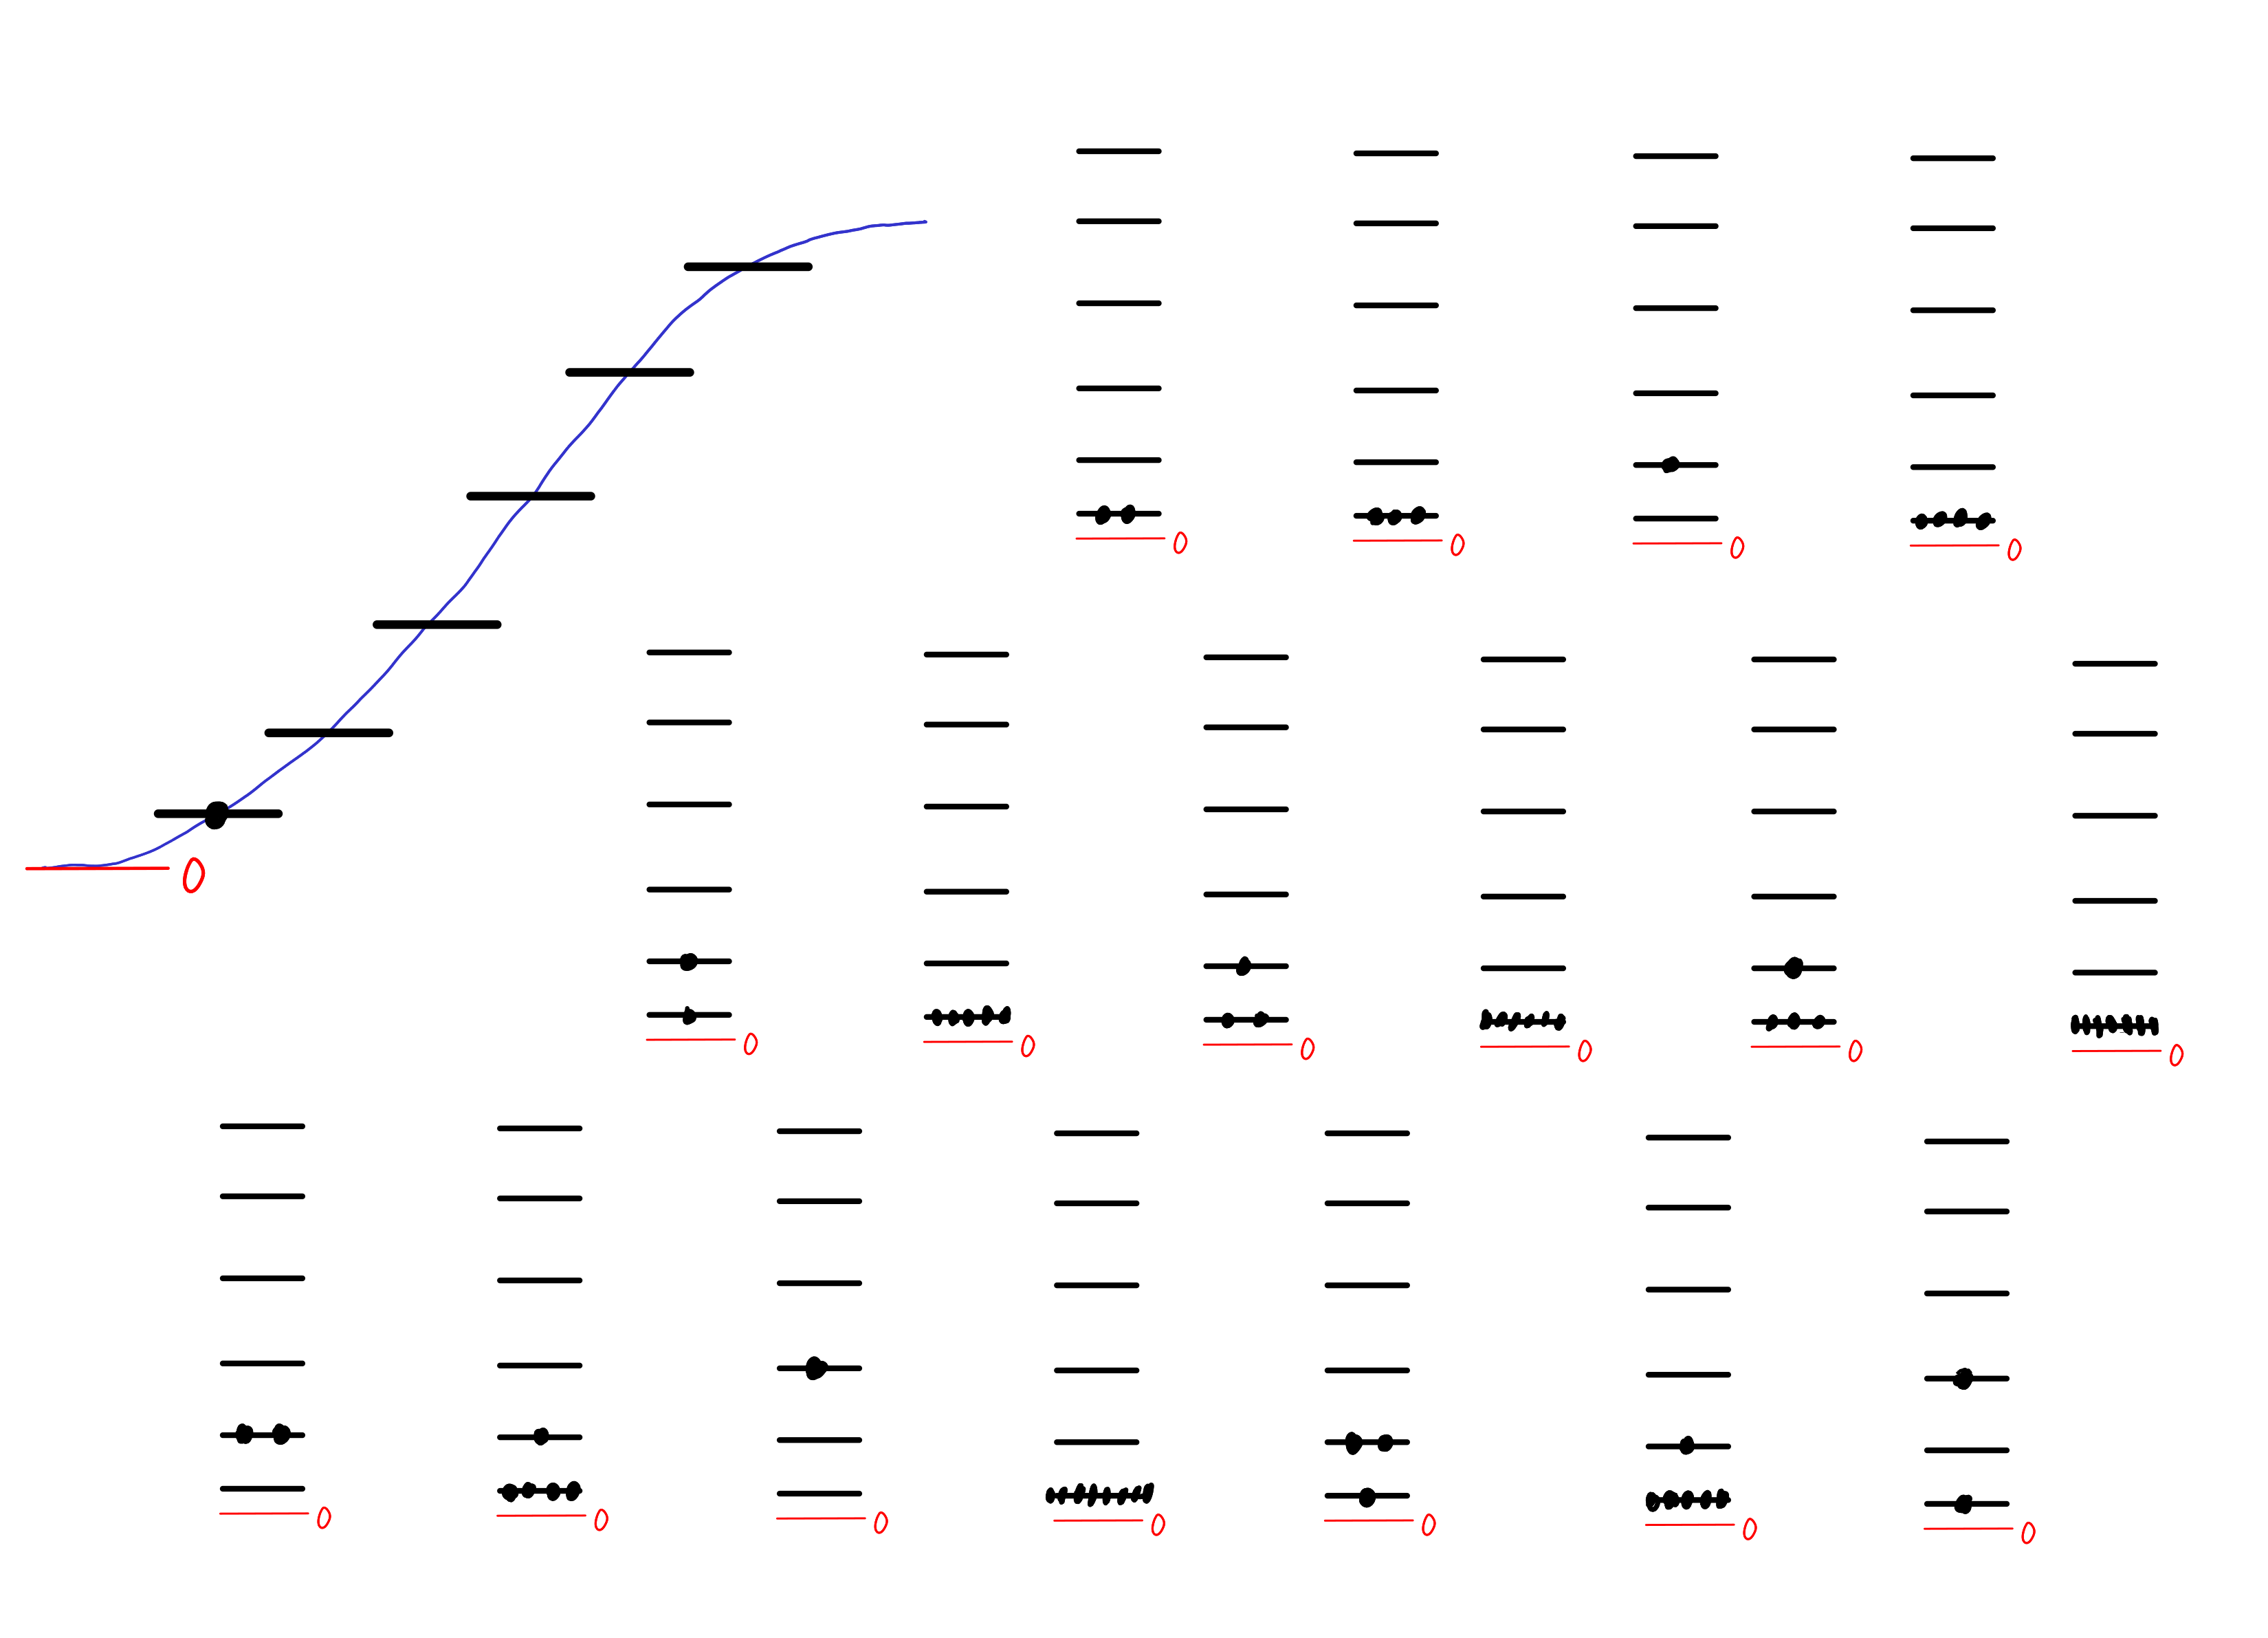
\includegraphics[width=\textwidth]{polymer_levels.png}
\end{figure}

\section{The VAMP Score}

For continuous systems, the Koopman operator will be infinite dimensional. To make use of the theory on a finite computer, we can just take the $n$ largest singular values of $\Kp$ and work with an approximation of the Koopman operator using only the top $n$ singular values and their corresponding singular functions.

The singular value decomposition can be written as a maximization problem.

% TODO: make sure to mention relevance of orthogonality

\section{VAMPNets}
\section{Extra Notes}

Ornstein Uhlenbeck in 2D ($k_x=k_y$). First two Koopman coordinates are $x$ and $y$.

Restricting to just these coordinates, is this the ``density matrix''?

$$
\rho=\begin{pmatrix}
	x & 0 \\
	0 & y
\end{pmatrix}
$$

with coordinate operators:

$$
\w{X} = \begin{pmatrix}
	1 & 0 \\
	0 & 0
\end{pmatrix}
\hspace{1cm}
\w{Y} = \begin{pmatrix}
	0 & 0 \\
	0 & 1
\end{pmatrix}
$$

so that $\langle \w{A} \rangle = \Tr\bk{\w{A}\rho}$


\end{document}
